The
\href{https://arstechnica.com/tech-policy/2023/03/silicon-valley-bank-shut-down-by-us-banking-regulators/}{collapse
of Silicon Valley Bank} has been breathtaking. There are already impacts
rippling outward from this that I've spotted on Mastodon. Quoting
@annmlipton@esq.social:
\url{https://esq.social/@annmlipton/110000882966755391} \#retoot:

\begin{figure}
\centering
\pandocbounded{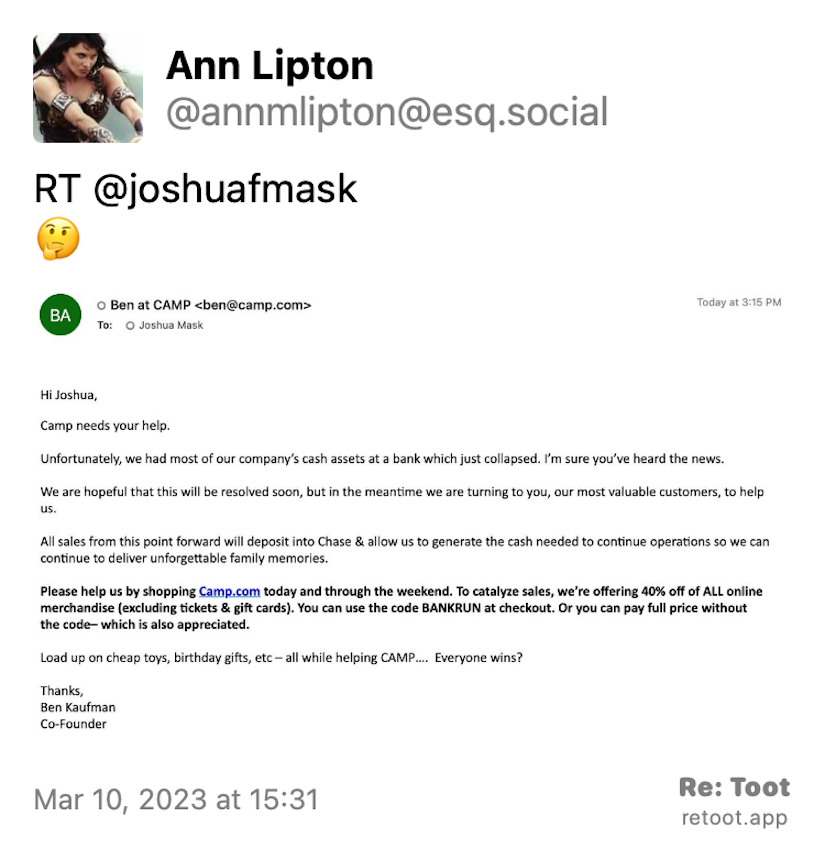
\includegraphics[keepaspectratio]{\%7B\%7Bsite.url\%7D\%7D/img/svb-ripple.jpg}}
\caption{Post by Ann Lipton. ``RT @joshuafmask 🤔'' The post contains an
image with no description. Posted on Mar 10, 2023 at 15:31}
\end{figure}

Businesses are already getting damaged by this. If that glimpse from
Mastodon wasn't enough, let us go ahead and look at this screen-cap from
the header to their home page at
\href{https://web.archive.org/web/20230310220216/https://camp.com/}{camp.com}
before their site went 503:

\begin{figure}
\centering
\pandocbounded{
\includegraphics[keepaspectratio]{\%7B\%7Bsite.url\%7D\%7D/img/svb-doom.jpg}}
\caption{OUR BANK JUST CLOSED - SO EVERYTHING IS ON SALE! 40\% OFF CODE:
BANKRUN}
\end{figure}

Businesses are having to hurriedly raise capital in any way they can.
Silicon Valley Bank was insured by FDIC, the Federal Deposit Insurance
Corporation. The problem is that insurance on accounts caps out at just
a quarter of a million dollars per account. If you're a startup with
millions or even billions in an account you quite likely watched your
operating cash get vaporized today.

I would start breaking out
\href{https://wiki.archiveteam.org/index.php/Wget_with_WARC_output}{wget
to write WARC archive files} of various sites as things are likely to
start disappearing. There is a proxy known as
\href{https://github.com/internetarchive/warcprox}{warcprox} that is a
bit of a kludge but it lets you capture things on the fly while you view
them so that you can have your own miniature web archive. With
supposedly thirty percent of YCombinator companies exposed to the SVB
failure likely being unable to make payroll in the next month
\href{https://news.ycombinator.com/item?id=35100743}{according to one
set of comments}, things are quite possibly going to start disappearing.

We can act like we can just ignore the pandemic situation but you can't
just skip the ``demobilization'' phase of an emergency. You can't just
play pretend like everything is magically normal again one day. The
clock didn't magically reset to 2019. The economy is still more fragile
than it should be and we're not on the same footing that we were
pre-pandemic. The Secretary also said she's got the department
\href{https://finance.yahoo.com/news/yellen-says-treasury-department-carefully-watching-crisis-at-a-few-banks-153243680.html}{monitoring
a few banks} in the wake of SVB's collapse so there is still a risk that
this financial problem may yet spread.
